\documentclass[11pt]{article}

\usepackage[letterpaper,margin=1in]{geometry}

\usepackage{akteach}
\usepackage{amsmath}
\usepackage{amssymb}
\usepackage{enumerate}
\usepackage{keystroke}

\usepackage{natbib}
\newcommand{\doi}[1]{\href{http://dx.doi.org/#1}{doi: #1}}

\lstset{
  language=Bash,
  basicstyle=\ttfamily,
  commentstyle=\color{blue},
  stringstyle=\color{black},
}

\begin{document}

\akteachheader{High-Performance Scientific Computing (MATH-GA 2011/ CSCI-GA 2945)}%
{Homework Set 1}
\akteachsubheader{Due: September 12, 2012 $\cdot$ Out: September 5, 2012 }

\smallskip
Welcome to this semester's high-performance computing (``HPC'') class!
Remember that this class is about \emph{you} and how much you learn.
Please let us (the instructors) know what we can do to improve your
experience.

\smallskip This first assignment is meant to get you familiar with the
mechanics of this class, from asking questions, to compiling and
running code, to turning in homework. It'll also provide some
practice with C code. If you're unfamiliar with C or the tools we are
using, expect to spend a fair bit of time \emph{now} to catch up.
This will ensure that you won't be lost once we get to more
complicated things. If you're already a skilled hacker on the other
hand, you should fly through this assignment.

\smallskip
After the description of the assignment, you will find a few pages
that describe tools and procedures. Please make sure to read and
follow those carefully.

\bigskip
\akteachprobhead{Problem 1: Sorting with trees}

Write a program to sort a sequence of numbers using a
\weblink{https://en.wikipedia.org/wiki/Binary_tree}{binary tree}.
Define a \texttt{struct} to represent each node in
the tree.

\begin{enumerate}[a)]
\item Read a number \texttt{n} from the command line.
\item Allocate an array of \texttt{n} integers. Using
  \weblink{https://www.gnu.org/software/libc/manual/html_node/ISO-Random.html}{\texttt{rand()}},
  fill it with \texttt{n} random integers. Make sure to use
  \texttt{srand()} to pick a seed, for reproducibility.
\item Build a binary tree from your array of numbers.
\item Output the sorted list to \texttt{stdout}, one integer
  per line.
\item Make sure you free all memory that you've allocated.
  (Yes, we will check!)
\item \label{part:tree-asymp}As an expression of \texttt{n}, what is the worst
possible runtime? What runtime do you expect typically?
What determines which case you fall into?
(Don't worry about constant factors or lower-order
terms in your expressions.)
\item \label{part:tree-runtime-discuss}Use this
\weblink{https://gist.github.com/3614336}{timing code}
to measure the run time you get for a range of list sizes.
Discuss how your observations match with your prediction
in part \ref{part:tree-asymp}).
\end{enumerate}

You will turn in your solution as a
`\weblink{https://en.wikipedia.org/wiki/Git_\%28software\%29}{\texttt{git}}'
repository (see below).
Your submission should be in a subdirectory `\texttt{problem-1}' and
should consist of at least these two files:

\begin{enumerate}
  \item Your program, which should be called `\texttt{tree-sort.c}'.

    If your implementation consists of more than this
    one file, you must also supply a
    `\weblink{https://en.wikipedia.org/wiki/Make_\%28software\%29}{\texttt{Makefile}}'
    that will build your program when `\texttt{make}' is entered.
    (If you have never heard of \texttt{make}, ignore it for now,
    we will get to it.)

  \item A plain text file `\texttt{discussion.txt}' containing
    your solution to parts \ref{part:tree-asymp})
    and \ref{part:tree-runtime-discuss}) as plain
    text. (i.e. not Word, PDF, or some such)

    Your answer to each subproblem should be about a short paragraph.
\end{enumerate}

\akteachprobhead{Problem 2: Matrix multiplication}

Write two codes to multiply matrices.
\begin{enumerate}[a)]
\item Read a number \texttt{n} from the command line.
  Allocate two (one-dimensional) arrays \texttt{A} and \texttt{B}
of \texttt{n}${}^2$ \texttt{double}s.  Fill them with random
numbers between 0.5 and 2.
\item \label{part:matmul}Viewing each of the one-dimensional arrays
  as a two-dimensional array in
  \weblink{http://en.wikipedia.org/wiki/Row-major_order}{column-major
  order}
  (see Figure \ref{fig:column-major}), we can now represent a matrix.
  Allocate a third array \texttt{C} and write a function to fill it
  with the product of the two matrices, according to this procedure:
  \begin{lstlisting}
    for i = 1 to n
      for j = 1 to n
        for k = 1 to n
          C[i,j] = A[i,k] * B[k,j]
        end
      end
    end
  \end{lstlisting}
  (Note that you'll have to translate the two indices into one. You
  might want to consider using a macro for this type of access.)

\item \label{part:mat-output}Write a subroutine that outputs a matrix to the screen
  as a square array as a human would write it.
  Use this subroutine to check your work in part \ref{part:matmul})
  on a small example.
  Output five characters per number (plus a space), and make sure the
  columns of your output line up.

\item Now write a subroutine that transposes a matrix, i.e. that
  computes
  \begin{lstlisting}
    for i = 1 to n
      for j = 1 to n
        D[i,j] = A[j,i]
      end
    end
  \end{lstlisting}
  Realize that changing the matrix from column- to `row-major' storage
  order is the same thing as transposition.

\item \label{part:matmul-t} Now make a new function
  that also performs matrix multiplication, but accepts
  \texttt{A} in row-major order.

  Write some code to check that the results from this routine agree
  with your existing code from part \ref{part:matmul}).

\item \label{part:mat-perf}Measure the run time of your code for parts \ref{part:matmul})
  and \ref{part:matmul-t}) for a few values of $n$. If one is faster,
  for what matrix size \texttt{n} does it become efficient to change the
  storage order, assuming \texttt{A} is always given in the `slow'
  order? (Use the timing code from the first problem. You will also
  need to time your transposition routine.)

  Also try different optimization levels by giving flags \texttt{-O0},
  \texttt{-O1}, \texttt{-O2}, \texttt{-O3} to the compiler.  Also try
  \texttt{-ffast-math}, which sets a number of potentially dangerous
  options, and the safer \texttt{-fassociative-math}.  Read up on
  their meanings.

  Write up your findings.
\end{enumerate}

Please submit the following, in the subdirectory `\texttt{problem-2}'
of your repository:
\begin{enumerate}
  \item A program \texttt{matmul.c} solving the above assignment.
  \texttt{main()} in this file may \emph{only} consist of calls to
  independent functions \verb|part_a|, \verb|part_b|, so that each
  part can be run in isolation by commenting out the other parts.

  You will need subroutines for at least parts \ref{part:matmul}),
  \ref{part:mat-output}), and \ref{part:matmul-t}).

  Again, please make sure that you free all the memory you allocate.
  \item A plain text file \texttt{part-\ref{part:mat-perf}.txt}
  with your measurements and discussion from part
  \ref{part:mat-perf}).
\end{enumerate}

\begin{figure}

\begin{center}
  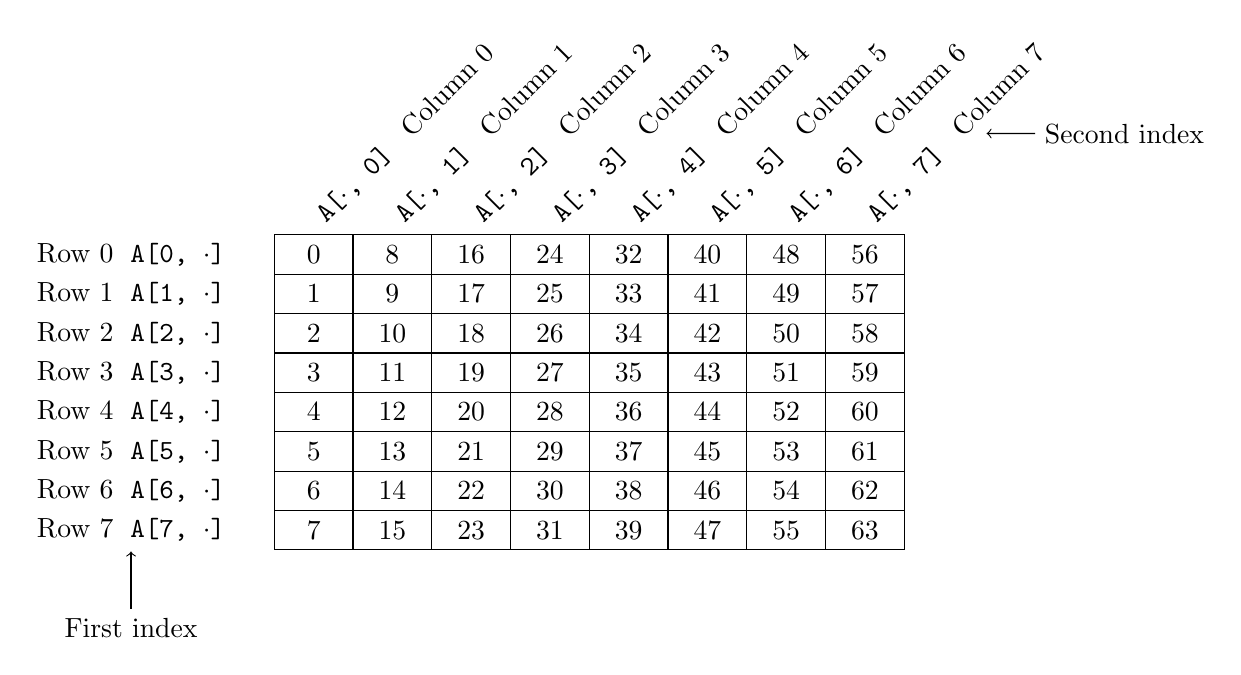
\begin{tikzpicture}[yscale=-0.5]
    \foreach \i in {0,1,...,7}
      \foreach \j in {0,1,...,7}
      {
        \draw (\i,\j) rectangle +(1,1) node [pos=0.5] {
          \pgfmathtruncatemacro{\res}{\i*8+\j}\res
        };
      }
    \foreach \i in {0,1,...,7}
    {
      \node (rowmark\i) at (-0.5,\i+0.5) [anchor=east]
      { Row \i \; \texttt{A[\i, $\cdot$]} } ;
    }
    \foreach \j in {0,1,...,7}
    {
      \node (colmark\j) at (\j+0.5, -0.25) [anchor=west,rotate=45]
      { \texttt{A[$\cdot$, \j]} \; Column \j } ;
    }
    \draw [<-] (colmark7) -- ++(1,0) node [anchor=west] {Second index};
    \draw [<-] (rowmark7) -- ++(0,2) node [anchor=north] {First index};
  \end{tikzpicture}
\end{center}

\caption{Column-major matrix layout. The numbers in the cells
represent linear array indices.}
\label{fig:column-major}
\end{figure}

\clearpage
% -----------------------------------------------------------------------------
\akteachheader{Machines and Homework Submission}{Helpful Hints}

% -----------------------------------------------------------------------------
\subsection*{Getting Help}

If you are having technical trouble, if some instructions here fail to
work for you, or if things just seem confusing, don't despair: There's
plenty of help available.

First of all, please make sure you are subscribed to the class mailing
list. Someone might have had the same problem as you (and ideally
already solved it). If you're either officially signed up in Albert or
added your name to the sign-up sheet in class, you should already be
on the list--you can tell by whether you've received a welcome email
on Wednesday night.  If you aren't subscribed, you may do so yourself
at \weblink{http://lists.tiker.net/listinfo/hpc12}{the list's web
page}. The list has
\weblink{http://lists.tiker.net/private/hpc12/}{archives} where you
can check if you've missed anything important.

If your problem concerns the NYU HPC machines (which we'll use later
in the class), try checking the
\weblink{https://wikis.nyu.edu/display/NYUHPC}{NYU HPC Wiki}.  If that
(and perhaps a bit of Googling around) doesn't answer your question,
send email to
\begin{quote}
  \href{mailto:hpc12@tiker.net}{\texttt{hpc12@tiker.net}}.
\end{quote}

If you would like to discuss a technical issue (i.e. one that isn't
directly related to you), please do not email us (the instructors)
directly--we'll just tell you to ask on the list.  So instead, please
send a message to the mailing list, where we (and your peers) will be
more than happy to assist.  Thanks!

Again, welcome, and we hope you'll have an enjoyable and worthwhile
experience in this class.

\begin{note}
All work in this class will be UNIX-based.  We've provided a virtual
machine (`VM') that lets you use all the technologies we'll touch on
in this class. (C99, OpenMP, MPI, OpenCL) Note that things won't go as
fast in the VM as on `real hardware', but it's more than enough for
coding and debugging.

At some later point, we will also introduce you to the usage of the
shared-use clusters maintained by the \weblink{http://hpc.nyu.edu}{NYU
HPC group}.
\end{note}

First, install \weblink{http://virtualbox.org}{VirtualBox} and run it.
Then, download the following machine image:
\begin{quote}
  \url{http://bit.ly/hpc12-vm}
\end{quote}
If you are \emph{certain} that you are running a 64-bit operating
system, you may instead grab this image (it will run slightly faster
and also have the Intel OpenCL implementation):
\begin{quote}
  \url{http://bit.ly/hpc12-vm-64}
\end{quote}

These files are about 2 GB in size each, so it'll take a while to download.
(You'll only need one of them!)
If possible, grab it at NYU using a wired connection.
If your browser didn't do this for you, you may have to rename the
file so that it has a \texttt{.ova} file extension.
If you're unable to download, ask one of the instructors--we have a
USB stick with the image and VirtualBox (the software that runs it).

Once downloaded, click ``File | Import Appliance...'' to import the VM
into VirtualBox.  This takes a few minutes, after which you can delete
the file you downloaded.

\begin{note}
Once the VM is done importing, you should change it to use the
number of cores actually present in your machine. To do so,
right-click the entry `HPC Class Linux VM', then click
`Settings\dots', `System', and `Processor'. Then slide the
`Processor(s)' slider to the number of cores you'd like to
use. Avoid the red area.
\end{note}

You can then start the VM by double-clicking on `HPC Class Linux VM',
and you'll be presented with a Linux desktop.  You can make that
desktop full-screen, if you wish.

You can of course also use your own Linux (or OS/X) machine, but then
you're on your own with respect to installing the software that we'll
need.

% -----------------------------------------------------------------------------
\subsection*{Using Unix and the command line}

While the VM provides a friendly point-and-click interface, we will be
doing most of our work on the command line, which you can get by
double-clicking the `Terminal' icon on the desktop (and by many other
ways).

While we hope you'll eventually agree that the command line is great
for doing development work, it can be a bit intimidating at first.

Once you click the icon, you're greeted with a `prompt':
\begin{lstlisting}
hpc@dizzy:~$
\end{lstlisting}
and a cursor next to it. \texttt{hpc} is your user name,
\texttt{dizzy} is the name of the VM. \texttt{\~} is a shorthand for
your home directory, and this spot in the prompt generally shows the
current working directory you're in. \verb|$| finally is the prompt
itself.

\begin{note}
We'll be a bit briefer from here on out.  From now on, the dollar
sign ``\texttt{\$}'' represents the command prompt.
\end{note}

If you are unsure of what to type next, consider taking a look at
\weblink{http://www.ee.surrey.ac.uk/Teaching/Unix/}{a
friendly Unix tutorial} (recommended). (Googling for ``unix tutorial''
gives plenty more options.)

You will also need to edit plain text files. There are plenty of text
editors that work in the terminal (nano, emacs, vim, all installed in
the VM). If you've never used any of these, the `Text Editor' link on
the desktop of the VM provides  provides a simple text editor that's
not scary and works a bit like Microsoft Word.  You can also start
that editor from the prompt:
\begin{lstlisting}
$ gedit filename.c
\end{lstlisting}
(Remember that you don't have to type the \verb|$|.)

Also, note that you will get a
\weblink{http://en.wikipedia.org/wiki/Bash_(Unix_shell)}{bash} shell
by default. If you are used to the C shell, ask us on how to change
that. (If this was mumbo-jumbo to you, forget about it.)

% -----------------------------------------------------------------------------
\subsection*{Using \texttt{git} for Homework and Collaboration}

We expect you to use the
\weblink{http://en.wikipedia.org/wiki/Distributed_revision_control}{distributed
version control} system \weblink{http://git-scm.org}{git} for
developing and turning in solutions to your homework. Like compilers,
debuggers, and build tools, version control systems are central to
most present-day software development. By having you use \texttt{git},
we hope to be able to give you some familiarity with such tools.

Along with the tool itself, we will use a central collaboration space,
\url{http://forge.tiker.net}, which works like the big, public
development hubs Github, Google Code, or SourceForge. You will set up
an account there and create a new ``project'' for every assignment
(and your final project). The collaboration space provides the
following functions in our class:
\begin{itemize}
  \item We will grade what is on \texttt{forge} after the homework
  deadline. As a result, you definitely want to upload your finished
  assignment.
  \item It will allow you to collaborate on your final project with a friend.
  \item If you are having an issue with your current code, you may
  upload it and ask the instructors to view it on \texttt{forge}.
  \item It provides an easy conduit to get code from the HPC clusters
  onto another machine and back.
\end{itemize}

\begin{note}
Your account on \texttt{forge} is initially limited to
about 50 megabytes, with more available if needed. Please do not check
in large data files before discussing your needs with Andreas.

Your accounts on \texttt{forge} and the data you store there will be
removed on February 1, 2013. Please back up your code and data before
this date.
\end{note}
Git is preinstalled on our virtual machine.

To start, open a terminal (use the icon on the VM desktop) and inform
\texttt{git} of your name and email address:
\begin{lstlisting}
$ git config --global user.name "Your Name"
$ git config --global user.email you@yourdomain.example.com
\end{lstlisting}

To access the class-wide collaboration space, go to
\url{http://forge.tiker.net}. Click ``Sign in or create account''.
Please use your NetID as your user name. The system will confirm your
email address by sending you a confirmation key. You can use the
web browser in the VM to do this.

\begin{note}
We have found that these confirmation emails often get flagged as spam
by a variety of spam filters. Please check your spam folder if the
email doesn't seem to have arrived within a few minutes.
\end{note}

Once you complete this
verification step, fill out your name, password, and click ``Enable my
Account''. Please do \emph{not} use a valuable password here, in
particular \emph{not} your NYU-wide one. You are now logged into
\texttt{forge.tiker.net}.

Next, type
\begin{lstlisting}
$ ssh-keygen
Generating public/private rsa key pair.
# Just hit Enter for this prompt.
Enter file in which to save the key (/home/hpc/.ssh/id_rsa): 
Created directory '/home/hpc/.ssh'.
# Pick a password here, or leave empty if you're feeling lucky.
Enter passphrase (empty for no passphrase): 
Enter same passphrase again: 
Your identification has been saved in /home/hpc/.ssh/id_rsa.
Your public key has been saved in /home/hpc/.ssh/id_rsa.pub.
The key fingerprint is:
df:0d:72:0b:19:f6:c4:ec:10:8b:0d:45:69:84:55:0a hpc@dizzy
The key's randomart image is:
+--[ RSA 2048]----+
|        E**o.    |
|        .=o*     |
|        ..B +    |
|         . B     |
|        S + =    |
|         . = +   |
|          . o .  |
|                 |
|                 |
+-----------------+
$ cat $HOME/.ssh/id_rsa.pub
\end{lstlisting}
(Again, don't type the \verb|$| signs\dots)
This will print a few lines (technically, just one wrapped line) that
looks like this:
\begin{lstlisting}
ssh-rsa AAAABw...vM3XdIbZWwmXH/iNbFWEhZw== hpc@dizzy
\end{lstlisting}
Once you are logged into \texttt{forge}, click your name in the top
left corner. Click ``Update your account'' on the left and then paste
the line returned above into the field that says ``Add public key''.
Click ``Update your Account''. The key update may take up to two
minutes to fully complete, so if the `\texttt{git push}' below fails,
wait for two minutes, and then try again.
This completes the setup steps that are only required once.

Next, create a directory for your homework submission.
\begin{lstlisting}
$ mkdir hw1
$ cd hw1
$ git init
Initialized empty Git repository in /home/hpc/hw1/.git/
$ git status
On branch master

Initial commit

nothing to commit (create/copy files and use "git add" to track)
\end{lstlisting}
The `\texttt{init}' command told \texttt{git} that you would like it to
manage this directory. Now go ahead and start on your project.
Once you've gotten to a point that you would like to save, say
\begin{lstlisting}
$ git add file1.c file2.txt
$ git commit
\end{lstlisting}
\texttt{git} will ask you for a commit message.

After your first commit, let's establish a connection between your
local repository and a repository on forge.  To do this, navigate to
\url{http://forge.tiker.net/} (or click on ``Project List'' if you're
already there) and, once there, click on ``Create Project''. You may
choose a name for the new repository, as well as a ``shortname'' (i.e.
Unix-level name).

\begin{note}
To make sure we find your homework, please choose
this shortname following the pattern ``\texttt{hpc12-hw1-netid123}''.
If you don't, we likely won't find your submission!
\end{note}

For the ``Project Creation Key'', enter ``\texttt{nyuhpc12}'' and make
sure the ``Private repository'' box is checked. If necessary, you may
also add co-owners and collaborators by their NetID. (Note that you're
free to discuss homework with your peers, but you \emph{must} write
your own code. In other words, collaboration will likely only become
relevant once we get to the final project.)
Once you click ``Create Project'', your repository is created on
forge.  To establish the link with your local one, say
\begin{lstlisting}
$ git remote add forge ssh://git@forge.tiker.net:2234/<shortname>.git
\end{lstlisting}

You may then say
\begin{lstlisting}
$ git push forge master
# If you entered a password in ssh-keygen above, you'll be asked
# to enter it again now.
Counting objects: 34, done.
Delta compression using up to 8 threads.
Compressing objects: 100% (21/21), done.
Writing objects: 100% (34/34), 8.25 KiB, done.
Total 34 (delta 12), reused 30 (delta 11)
To ssh://git@forge.tiker.net:2234/hw1-ak177.git
 * [new branch]      master -> master
\end{lstlisting}
to upload your commits.

You may also navigate to \url{http://forge.tiker.net}, pick your
project from the list, navigate to the ``Source'' tab and verify that
the right version of the code is checked in.

From here on out, the cycle of add/commit/push just repeats.  Please
also take a look at the
\weblink{http://www.kernel.org/pub/software/scm/git/docs/gittutorial.html}{git
tutorial}. You should at least be familiar with the usage of the
commands
\begin{itemize}
  \item \texttt{git status}
  \item \texttt{git add}
  \item \texttt{git commit}
  \item \texttt{git log}
  \item \texttt{git diff}
\end{itemize}
One piece of advice: Commit frequently--at least once
for every milestone you complete along the way. This allows you
to go back to a working version if you've made changes that you would
like to get rid of.

\end{document}
